\documentclass[a4paper,12pt]{article}
\usepackage[utf8]{inputenc}
\usepackage{amsmath}
\usepackage{bm} % to get bold epsilon
\usepackage{amssymb}
\usepackage{comment}
\usepackage{graphicx}
\usepackage{xcolor}
\usepackage[left=1.5cm, right=1.5cm, top=2cm, bottom=2cm]{geometry}
\title{\textbf{COM 5120 Communication Theory}}
\author{\textbf{Practice \#3}}
\date{No need to turn it in, this is for practice purpose only.  \\
Practice and get familiar with the questions are encouraged. \\ 
Some types of the questions might appear on the test. \\}
\begin{document}
    \maketitle
    % \textit{Note: }There are \textbf{6} problems with total 100 points within \textbf{3} pages, please write your answer with detail in the answer sheet.
    % {\bf No credit without detail.  No calculator. Closed books.}
    \begin{enumerate}
    %%%%%%%%%%%%%%%%%%%%%%%%%%%%%%
        \item 
            % 1. (6.40)
            A discrete memoryless source produces outputs $\{a_1, a_2, a_3, a_4, a_5 \}$. The corresponding output probabilities are $0.8$, $0.1$, $0.05$, $0.04$, and $0.01$. \\
            (a) Design a binary Huffman code for the source. Find the average codeword length. Compare it to the minimum possible average codeword length. \\
            (b) Assume that we have a binary symmetric channel with crossover probability $\epsilon = 0.3$. Is it possible to transmit the source reliably over the channel? Why? \\
            (c) Is it possible to transmit the source over the channel employing Huffman code designed for single source outputs? \\ \\
            \textbf{Solution:} \\
            \textbf{(a)} The Huffman tree is shown in Figure 1: \\ 
            \begin{figure}[h]
            	\centering
            	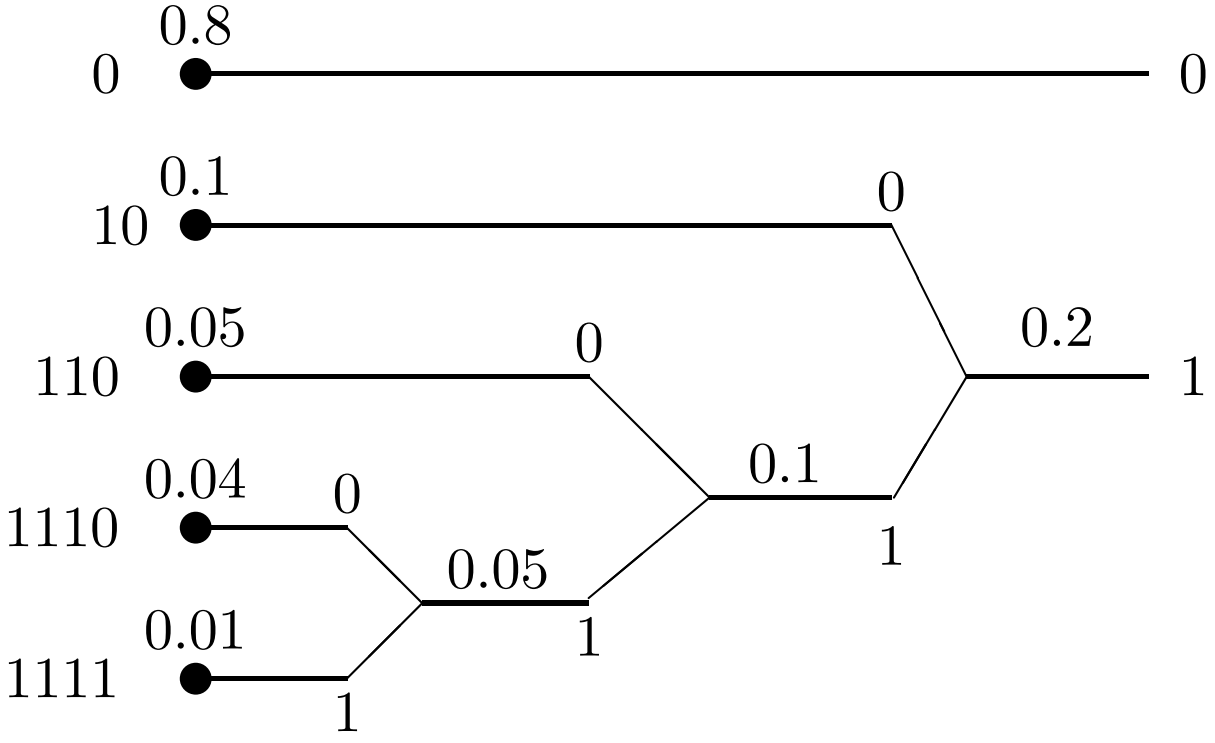
\includegraphics[scale=0.35]{Practice3-1-1.png}
            	\caption{Huffman tree}
            % 	\label{fig}
            \end{figure} \\
            The average codeword length is $\Bar{R} = 0.8 \times 1 + 2 \times 0.1+ 3 \times 0.05 + 4 \times (0.01 + 0.04) = 1.35$ and the minimum possible average codeword length given by the entropy is $H(X) = \sum p_i \log_2 p_i = 1.058$. Obviously $H(X) < \Bar{R}$ as expected. \\ 
            \textbf{(b)} The capacity of the channel is $C = 1 - H_b(0.3) = 0.1187$. Since $H(X) > C$ it is not possible to transmit the source reliably. \\
            \textbf{(c)} No, since $\Bar{R} > C$.
            \begin{flushright}
                $\blacksquare$
            \end{flushright}
    %%%%%%%%%%%%%%%%%%%%%%%%%%%%%%
        \item
            % 2. (6.43)
            For the channel shown in Figure 2, find the channel capacity and the input distribution that achieves capacity. 
            \begin{figure}[h]
            	\centering
            	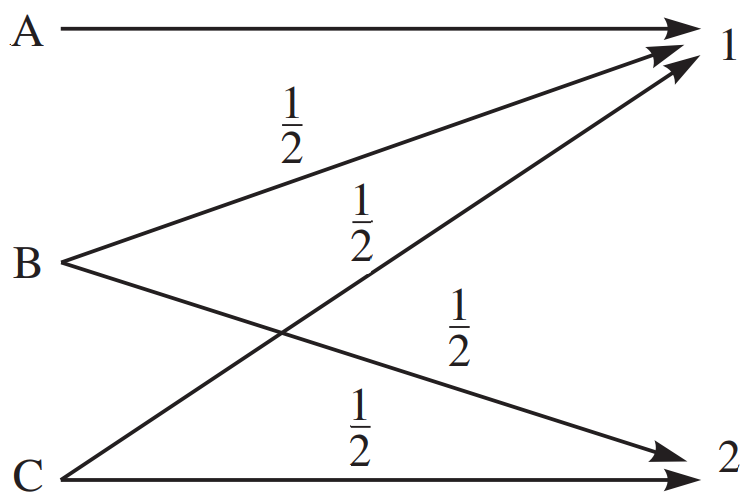
\includegraphics[scale=0.35]{Practice3-2-1.png}
            	\caption{channel model}
            % 	\label{fig}
            \end{figure} \\ 
            \textbf{Solution:} \\
            By symmetry of the inputs \textbf{B} and \textbf{C}, their probabilities have to be equal. Therefore we may assume that 
            % $P(A) = 1 - p$, $P(B) = P(C) = p/2$. 
            $$ 
            \begin{aligned}
                & P(A) = 1 - p \\
                & P(B) = P(C) = p/2
            \end{aligned}
            $$ \\
            We then have 
            % $P(Y = 1) = 1 - p + p/2$ and $P(Y = 0) = p/2$, 
            $$ 
            \begin{aligned}
                & P(Y = 1) = 1 - p + p/2 \\
                & P(Y = 0) = p/2
            \end{aligned}
            $$ \\
            thus $H(Y) = H_b(p/2)$. We also note that 
            % $H(Y|X = A) = 0$ and $H(Y|X = B) = H(Y|X = C) = 1$, 
            $$ 
            \begin{aligned}
                & H(Y|X = A) = 0 \\
                & H(Y|X = B) = H(Y|X = C) = 1
            \end{aligned}
            $$ \\
            hence $$H(Y|X) = (1 - p) \cdot H(Y|X = A) \cdot 0 + p/2 \cdot H(Y|X = B) \cdot 1 + p/2 \cdot H(Y|X = C) \cdot 1 = p$$
            Therefore, 
            \begin{align*}
                C &= \max_{p} I(X;Y) \\
                  &= \max_{p} H(Y) - H(Y|X) \\
                  &= \max_{p} H_b(p/2) - p
            \end{align*}
            straightforward differentiation results in 
            \begin{align*}
                -\frac{1}{2} \log_2 e \ln \frac{p/2}{1 - p/2} - 1 = 0
            \end{align*}
            resulting in 
            \begin{align*}
               & p = 0.4 \\ 
               & C = H_b(0.2) - 0.4 = 0.3219
            \end{align*}
            \begin{flushright}
                $\blacksquare$
            \end{flushright}
    %%%%%%%%%%%%%%%%%%%%%%%%%%%%%%
        \item
            % 3. (6.56)
            A telephone channel has a bandwidth $W = 3000$ Hz and a signal-to-noise power ratio of $400$ ($26$ dB). Suppose we characterize the channel as a band-limited AWGN waveform channel with $P_{av}/W \cdot N_0 = 400$. Determine the capacity of the channel in bits per second. \\ \\ 
            \textbf{Solution:} \\
            The capacity of the continuous-time channel is given by relation (6.5-43) on p. 366 which gives: 
            \begin{align*}
                C = W \textcolor{red}{\log_2} \left( 1 + \frac{P_{av}}{W \cdot N_0} \right) = 25.9 \;\; \text{Kbits/sec}
            \end{align*}
            \begin{flushright}
                $\blacksquare$
            \end{flushright}
            % \newpage
    %%%%%%%%%%%%%%%%%%%%%%%%%%%%%    
        \item 
            % 4. (6.60)
            \textcolor{red}{Figure 3} illustrates a binary erasure channel with transition probabilities $P(1|1) = 1 - p$ and $P(e|0) = p$. The probabilities for the input symbols are $P(X = 0 = \alpha$ and $P(X = 1) = 1 - \alpha$.
            (a) Determine the average mutual information $I(X;Y)$ in bits. \\ 
            (b) Determine the value of $\alpha$ that maximizes $I(X;Y)$, i.e. the channel capacity $C$ in bits per channel use, and plot $C$ as a function of $p$ for the optimum value of $\alpha$. \\
            (c) For the value of $\alpha$ found in part (b), determine the mutual information $I(x;y) = I(0;0)$, $I(1;1)$, $I(0;e)$ and $I(1;e)$, where $I(x;y) = \textcolor{red}{\log_2} \frac{P[X = x, Y = y]}{P[X = x]P[Y = y]}$
            % \begin{align*}
            %     I(x;y) = \log \frac{P[X = x, Y = y]}{P[X = x]P[Y = y]}
            % \end{align*}
            \begin{figure}[h]
                \centering
                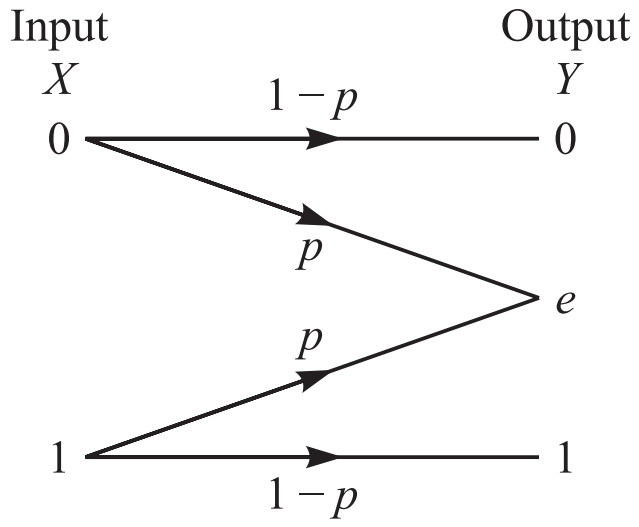
\includegraphics[scale=0.4]{Practice3-4-1.png}
                \textcolor{red}{\caption{binary erasure channel}}
                % \label{fig:my_label}
            \end{figure} \\ 
            \textbf{Solution:}
            \begin{align*}
                & P(X = 0) = a, \;\;\;\;\;\;\;\;\; P(Y = 0) = (1 - p) \cdot a \; \\
                & P(X = 1) = 1 - a, \;\;\; P(Y = 1) = (1 - p)(1 - a) \\
                & P(Y = e) = P(1 - a + a) = p \;
            \end{align*}
            \textbf{(a)} 
            \begin{align*}
                I(X;Y) &= \sum_{i = 1}^{2} \sum_{j = 1}^{3} P(y_j | x_i)P(x_i) \textcolor{red}{\log_2} \frac{P(y_j | x_i)}{P(y_j)} \\ 
                       &= a \cdot (1 - p) \textcolor{red}{\log_2} \frac{1 - p}{a \cdot (1 - p)} + a \cdot p \textcolor{red}{\log_2} \frac{p}{p} + (1 - a) \cdot (1 - p) \textcolor{red}{\log_2} \frac{1 - p}{(1 - a)(1 - p)} \\ 
                       &= -(1 - p) \cdot \left(a \textcolor{red}{\log_2} a + (1 - a) \textcolor{red}{\log_2} (1 - \textcolor{red}{a}) \right) \\ \\
                \text{Note that the term} & \;\; -\left(a \textcolor{red}{\log_2} a + (1 - a) \textcolor{red}{\log_2} (1 - \textcolor{red}{a}) \right) \;\; \text{is the entropy of the source.}
            \end{align*}
            % Note that the term $-\left(a \textcolor{red}{\log_2} a + (1 - a) \textcolor{red}{\log_2} (1 - \textcolor{red}{a}) \right)$ is the entropy of the source.
            \textbf{(b)} 
            The value of a that maximizes $I(X;Y)$ is found from:
            \begin{align*}
                & \Rightarrow \frac{dI(X;Y)}{da} = 0 \\ 
                & \Rightarrow \textcolor{red}{\log_2} a + \frac{a}{a} \textcolor{red}{\log_2} e - \textcolor{red}{\log_2} (1 - a) - \frac{1 - a}{1 - a} \textcolor{red}{\log_2} e = 0 \\ 
                & \Rightarrow a = \frac{1}{2}
            \end{align*}
            With this value of $a = \frac{1}{2}$, the resulting channel capacity is:
            \begin{align*}
                C = I(X;Y)|_{a = \frac{1}{2}} = 1 - p \;\; \text{bits/channel use} 
            \end{align*}
            \textbf{(c)} Since $I(X;Y) = \textcolor{red}{\log_2} \frac{P(y|x)}{P(y)}$ Hence:
            \begin{align*}
                & I(0;0) = \textcolor{red}{\log_2} \frac{1 - p}{(1 - p)/2} = 1 \\
                & I(1;1) = \textcolor{red}{\log_2} \frac{1 - p}{(1 - p)/2} = 1 \\
                & I(0;e) = \textcolor{red}{\log_2} \frac{p}{p} = 0 \\
                & I(1;e) = \textcolor{red}{\log_2} \frac{p}{p} = 0
            \end{align*}
            \begin{flushright}
                $\blacksquare$
            \end{flushright}
    %%%%%%%%%%%%%%%%%%%%%%%%%%%%%%%%%%%%%%%%%%%%%%    
        \item 
            % 5. (9.3)
            (a) Show that (Poisson sum formula).
            % $$x(t) = \sum_{k = - \infty}^{\infty} g(t)h(t - kT) \Rightarrow$$
            \begin{align*}
                x(t) = \sum_{k = - \infty}^{\infty} g(t)h(t - kT) 
                \Rightarrow X(f) = \frac{1}{T} \sum_{n = - \infty}^{\infty} H(\frac{n}{T}) G(f - \frac{n}{T})
            \end{align*}
            \textit{Hint}: Make a Fourier-series expansion of the periodic factor 
            $\sum_{k = - \infty}^{\infty} h(t - kT)$ \\ 
            (b) Using the result in (a), verify the following versions of the Poisson sum: 
            \begin{align*}
                & \sum_{k = - \infty}^{\infty} h(kT) = \frac{1}{T} \sum_{n = - \infty}^{\infty} H(\frac{n}{T}) \;\;\;\;\;\;\;\;\;\;\;\;\;\;\;\;\;\;\;\;\;\;\;\;\;\;\;\;\;\; \text{(i)} \\ 
                & \sum_{k = - \infty}^{\infty} h(t - kT) = \frac{1}{T} \sum_{n = - \infty}^{\infty} H(\frac{n}{T})e^{\frac{j2\pi nt}{T}} \;\;\;\;\;\;\;\;\;\;\;\;\;\;\;\; \text{(ii)} \\ 
                & \sum_{k = - \infty}^{\infty} h(kT) e^{-j2 \pi kTf} = \frac{1}{T} \sum_{n = - \infty}^{\infty}H(f - \frac{n}{T}) \;\;\;\;\;\;\;\;\;\;\; \text{(iii)} \\ 
            \end{align*}
            (c) Derive the condition for no intersymbol interference (Nyquist criterion) by using the Poisson sum formula. \\ \\
            \textbf{Solution:} \\
            \textbf{(a)} 
            Since $\sum_{k} h(t - kT) = u(t)$ is a periodic signal with period $T$. Hence, $u(t)$ can be expanded in the Fourier series: $$u(t) = \sum_{n = -\infty}^{\infty} u_{n}e^{j2 \pi nt/T}$$ where:
            \begin{align*}
                u_n &= \frac{1}{T} \int_{-T/2}^{T/2} u(t)e^{-2\pi nt/T}dt \\
                    &= \frac{1}{T} \int_{-T/2}^{T/2} \sum_{k = -\infty}^{\infty} h(t - kT) e^{-j2 \pi nt/T}dt \\
                    &= \sum_{k = -\infty}^{\infty} \frac{1}{T} \int_{-T/2}^{T/2} h(t - kT) e^{-j2 \pi nt/T} dt \\
                    &= \frac{1}{T} \int_{-\infty}^{\infty} e^{-j2 \pi nt/T}dt \\ 
                    &= \frac{1}{T} H(\frac{n}{T}) 
            \end{align*}
            Then:
            \begin{align*}
                &u(t) = \frac{1}{T} \sum_{n = -\infty}^{\infty} H(\frac{n}{T})e^{j2\pi nt/T} \\ 
                \Rightarrow \; & U(f) = \frac{1}{T} \sum_{n = -\infty}^{\infty} H(\frac{n}{T}) \delta(f - \frac{n}{T})
            \end{align*}
            Since $x(t) = u(t)g(t)$, it follows that $X(f) = U(f) * G(f)$ Hence: $$X(f) = \frac{1}{T} \sum_{n = -\infty}^{\infty} H(\frac{n}{T}) G(f - \frac{n}{T})$$ 
            \textbf{(b)} \\
            (i) $$\sum_{k = -\infty}^{\infty} h(kT) = u(0) = \frac{1}{T} \sum_{n = -\infty}^{\infty} H(\frac{n}{T})$$ 
            (ii) $$\sum_{k = -\infty}^{\infty} h(t - kT) = u(t) = \frac{1}{T} \sum_{n = -\infty}^{\infty} H(\frac{n}{T}) e^{j2\pi nt/T}$$ 
            (iii) 
            \begin{align*}
                & \text{Let} \;\; v(t) = h(t)\sum_{k = -\infty}^{\infty} \delta(t - kT) = \sum_{k = -\infty}^{\infty} h(kT) \delta(t - kT) \\ 
                & \text{Hence} \;\; V(f) = \sum_{k = -\infty}^{\infty} h(kT) e^{-j2\pi fkT} \\ 
                & \text{But} \;\; V(f) = H(f) * \text{Fourier transform of} \sum_{k = -\infty}^{\infty} \delta(t - kT) \\
                &   \;\;\;\;\;\;\;\;\;\;\;\;\;\;\;\; = H(f) * \frac{1}{T} \sum_{n = -\infty}^{\infty} \delta(f - \frac{n}{T}) \\
                &   \;\;\;\;\;\;\;\;\;\;\;\;\;\;\;\; = \frac{1}{T} \sum_{n = -\infty}^{\infty} H(f - \frac{n}{T})
            \end{align*}
            \textbf{(c)} 
            The criterion for no intersymbol interference is $\{ h(kT) = 0, k \neq 0 \; \text{and} \; h(0) = 1 \}$. If the above condition holds, then from (iii) above we then have:
            \begin{align*}
                \frac{1}{T} \sum_{n = -\infty}^{\infty} H(f - \frac{n}{T}) = \sum_{k = -\infty}^{\infty} h(kT)e^{-j2\pi fjT} = 1
            \end{align*}
            Conversely, if
            \begin{align*}
                \frac{1}{T} \sum_{n = -\infty}^{\infty} H(f - \frac{n}{T}) = 1, \forall f \\
                \Rightarrow \sum_{k = -\infty}^{\infty} h(kT) e^{j2\pi fkT} = 1, \forall f
            \end{align*}
            This is possible only if the left-hand side has no dependence on $f$, which means $h(kT) = 0, \; \text{for} \; k \neq 0$. Then $$\sum_{k = -\infty}^{\infty} h(kT) e^{-j2\pi fkT} = h(0) = 1$$
            \begin{flushright}
                $\blacksquare$
            \end{flushright}
    %%%%%%%%%%%%%%%%%%%%%%%%%%%%%%
        \item 
            % 6. (9.13)
            An ideal voice-band telephone line channel has a band-pass frequency-response characteristic spanning the frequency range $600-3000$ Hz. \\ 
            (a) Design an $M = 4$ PSK (quadrature PSK or QPSK) system for transmitting data at a rate of 2400 bits/s and a carrier frequency $f_c = 1800$ Hz. For spectral shaping, use a raised cosine frequency-response characteristic. Sketch a block diagram of the system and describe the functional operation of each block. \\
            (b) Repeat (a) for a bit rate $R = 4800$ bits/s and a \textcolor{red}{4-QAM }signal. \\ \\ 
            \textbf{Solution:} \\
            \textbf{(a)} 
            The bandwidth of the bandpass channel is: 
            \begin{align*}
                W = 3000 - 600 = 2400 \; \text{Hz}
            \end{align*}
            Since each symbol of the QPSK constellation conveys $2$ bits of information, the symbol rate of transmission is: 
            \begin{align*}
                R = \frac{1}{T} = \frac{2400}{2} = 1200 \; \text{symbols/sec}
            \end{align*}
            Thus, for spectral shaping we can use a signal pulse with a raised cosine spectrum and roll-off factor $\beta = 1$, since the spectral requirements will be:
            \begin{align*}
                \frac{1}{2T} (1 + \beta) = \frac{1}{T} = 1200 \; \text{Hz}
            \end{align*}
            Hence:
            \begin{align*}
                X_{rc}(f) = \frac{T}{2} \left[ 1 + \cos(\pi T |f|) \right] = \frac{1}{1200} \cos^2 \left( \frac{\pi|f|}{2400} \right)
            \end{align*}
            If the desired spectral characteristic is split evenly between the transmitting filter $G_T(f)$ and the receiving filter $G_R(f)$, then 
            \begin{align*}
                G_T(f) = G_R(f) = \sqrt{\frac{1}{1200}} \cos \left( \frac{\pi|f|}{2400} \right), \;\;\; |f| < \frac{1}{T} = 1200
            \end{align*}
            A block diagram of the transmitter is shown in figure 4.
            \begin{figure}[h]
            	\centering
            	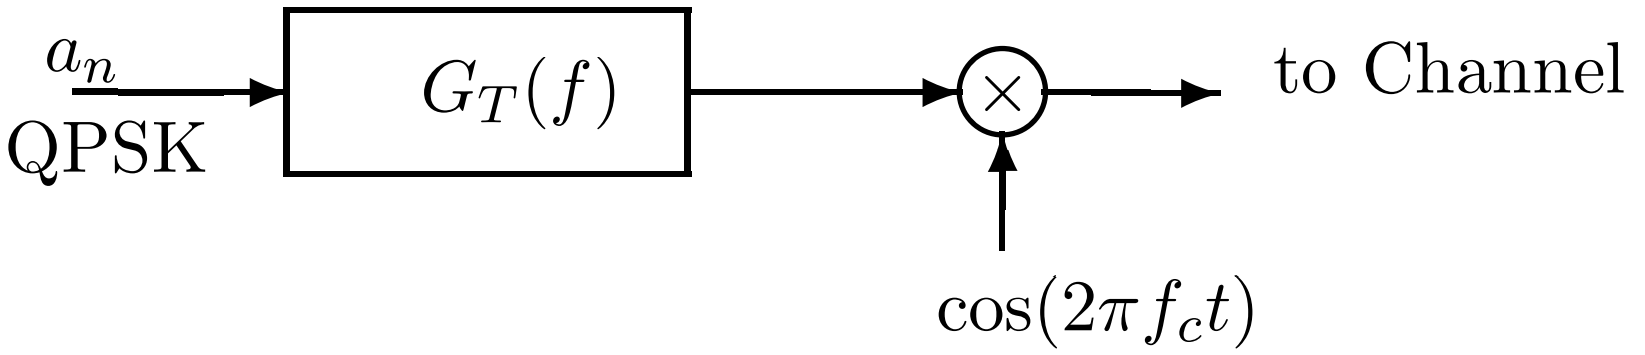
\includegraphics[scale=0.338]{Practice3-6-1.png}
            	\caption{block diagram of the transmitter}
            % 	\label{fig}
            \end{figure} 
            \newpage
            \textbf{(b)} 
            If the bit rate is $4800$ bps, then the symbol rate is
            \begin{align*}
                R = \frac{4800}{2} = 2400 \;\; \text{symbols/sec}
            \end{align*}
            In order to satisfy the Nyquist criterion, the the signal pulse used for spectral shaping, should have roll-off factor $\beta = 0$ with corresponding spectrum:
            \begin{align*}
                X(f) = T, \; |f| < 1200
            \end{align*}
            Thus, the frequency response of the transmitting filter is 
            \begin{align*}
                G_T(f) = \sqrt{T}, \; |f| < 1200
            \end{align*}
            \begin{flushright}
                $\blacksquare$
            \end{flushright}
    %%%%%%%%%%%%%%%%%%%%%%%%%%%%%%%%%%%%%%%%%%%%%%
        \item 
            % 7. (9.14)
            A voice-band telephone channel passes the frequencies in the band from $300$ to $3300$ Hz. It is desired to design a modem that transmits at a symbol rate of $2400$ symbols/s, with the objective of achieving $9600$ bits/s. \\
            Select an appropriate QAM signal constellation, carrier frequency, and the roll-off factor of a pulse with a raised cosine spectrum that utilizes the entire frequency band. \\
            Sketch the spectrum of the transmitted signal pulse and indicate the important frequencies. \\ \\ 
            \textbf{Solution:} \\
            The bandwidth of the bandpass channel is:
            \begin{align*}
                W = 3300 - 300 = 3000 \; \text{Hz}
            \end{align*}
            In order to transmit $9600$ bps with a symbol rate
            \begin{align*}
                R = \frac{1}{T} = 2400 \; \text{symbols/sec}
            \end{align*}
            the number of information bits per symbol should be
            \begin{align*}
                k = \frac{9600}{2400} = 4
            \end{align*}
            Hence, a $2^4 = 16$ QAM signal constellation is needed. The carrier frequency $f_c$ is set to $1800$ Hz, which is the mid-frequency of the frequency band that the bandpass channel occupies. If a pulse with raised cosine spectrum and roll-off factor $\beta$ is used for spectral shaping, then for the bandpass signal with bandwidth $W$:
            \begin{align*}
                & \frac{1}{2T}(1 + \beta) = \frac{W}{2} = 1500 \\
                & \Rightarrow \frac{1}{2} \cdot 2400 (1 + \beta) = 1500 \\
                & \Rightarrow 1 + \beta = \frac{1500}{1200} = 1.25 \\ 
                & \Rightarrow \beta = 0.25
            \end{align*}
            \newpage
            A sketch of the spectrum of the transmitted signal pulse is shown in \textcolor{red}{Figure 5}. 
            \begin{figure}[h]
            	\centering
            	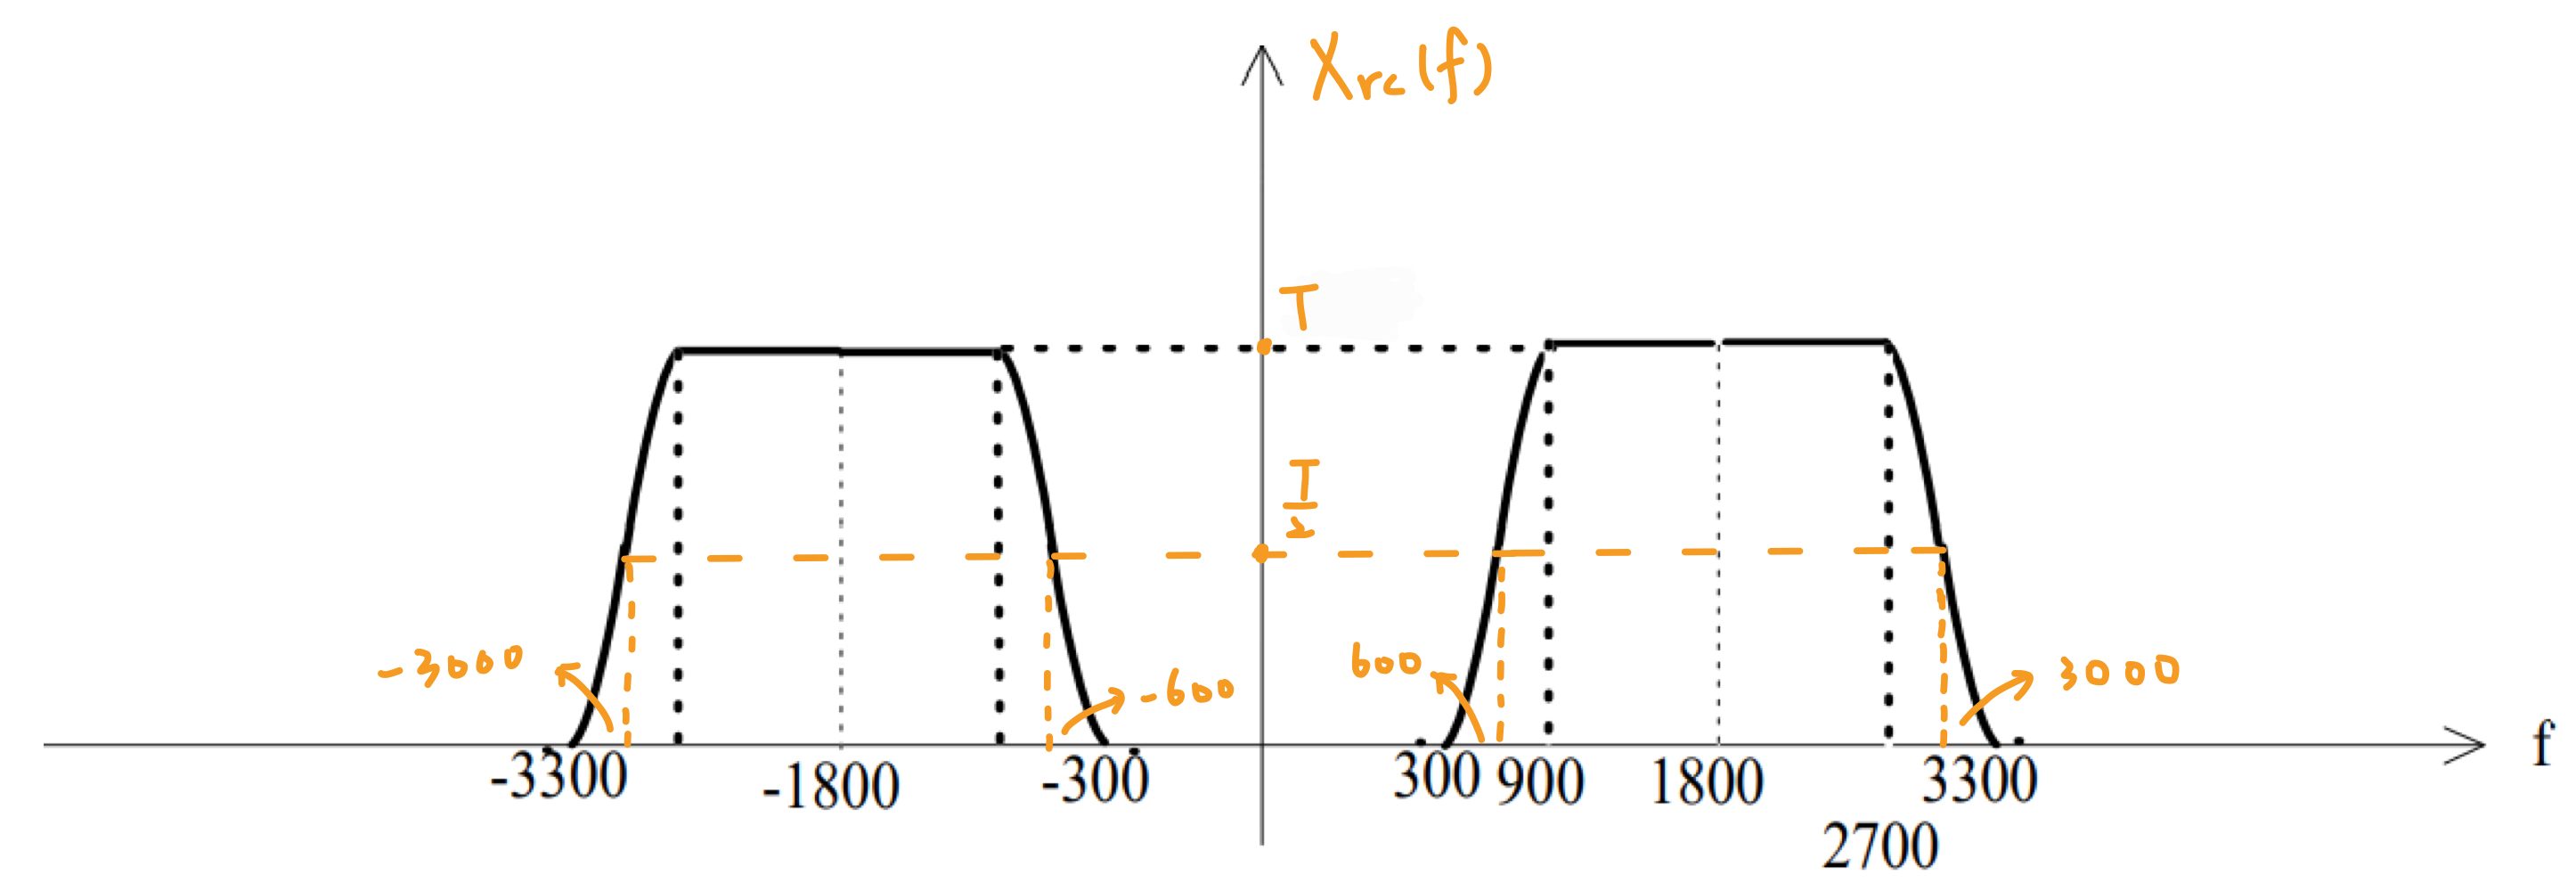
\includegraphics[scale=0.18]{Practice3-7-3.jpg}
            	\textcolor{red}{\caption{transmitter block diagram}}
            \end{figure}
            \begin{flushright}
                $\blacksquare$
            \end{flushright}
    %%%%%%%%%%%%%%%%%%%%%%%%%%%%%%%%%%%%%%%%%%%%%%
        \item 
            % 8. (Example 9.3-1)
            Suppose that the transmitter signal pulse $g(t)$ has duration $T$ and unit energy and the received signal pulse is $h(t) = g(t) + ag(t - T)$. \\ 
            Let us determine the equivalent discrete-time white noise filter model. The sampled autocorrelation function is given by 
            $$x_k = \left\{ 
            \begin{aligned}
                & a^* \;\;\;\;\;\;\;\;\;\;\; (k = -1) \\
                & 1 + |a|^2 \;\;\; (k = 0) \\ 
                & a \;\;\;\;\;\;\;\;\;\;\;\;\; (k = 1) \\
            \end{aligned}
            \right.
            $$
            \textbf{Solution:} \\ 
            The $z$ transform of $x_k$ is 
            \begin{align*}
                X(z) &= \sum_{k = -1}^{1} x_k z^{-k} \\
                     &= a^*z + (1 + |a|^2) + az^{-1} \\ 
                     &= (az^{-1} + 1)(a^*z + 1) 
            \end{align*}
            Under the assumption that $|a| < 1$, one chooses $F(z) = az^{-1} + 1$, so that the equivalent transversal filter consists of two taps having tap gain coefficients $f_0 = 1, f_1 = a$. Note that the correlation sequence $\{ x_k \}$ may be expressed in terms of the $\{ f_n \}$ as 
            \begin{align*}
                x_k = \sum_{n = 0}^{L - k} f_n^*f_{n + k}, k = 0, 1, 2, ..., L
            \end{align*}
            When the channel impulse response is changing slowly with time, the matched filter at the receiver becomes a time-variable filter. In this case, the time variations of the channel/matched-filter pair result in a discrete-time filter with time-variable coefficients. \\ 
            As a consequence, we have time-variable intersymbol interference effects, which can be modeled by the filter illustrated in Figure 9.3-3 (p. 628 in textbook), where the tap coefficients are slowly varying with time. 
            % \\ The discrete-time white noise linear filter model for the intersymbol interference effects that arise in high-speed digital transmission over nonideal band-limited channels will be used throughout the remainder of this chapter in our discussion of compensation techniques for the interference. In general, the compensation methods are called equalization techniques or equalization algorithms.
            % \begin{figure}[t]
            %     \centering
            %     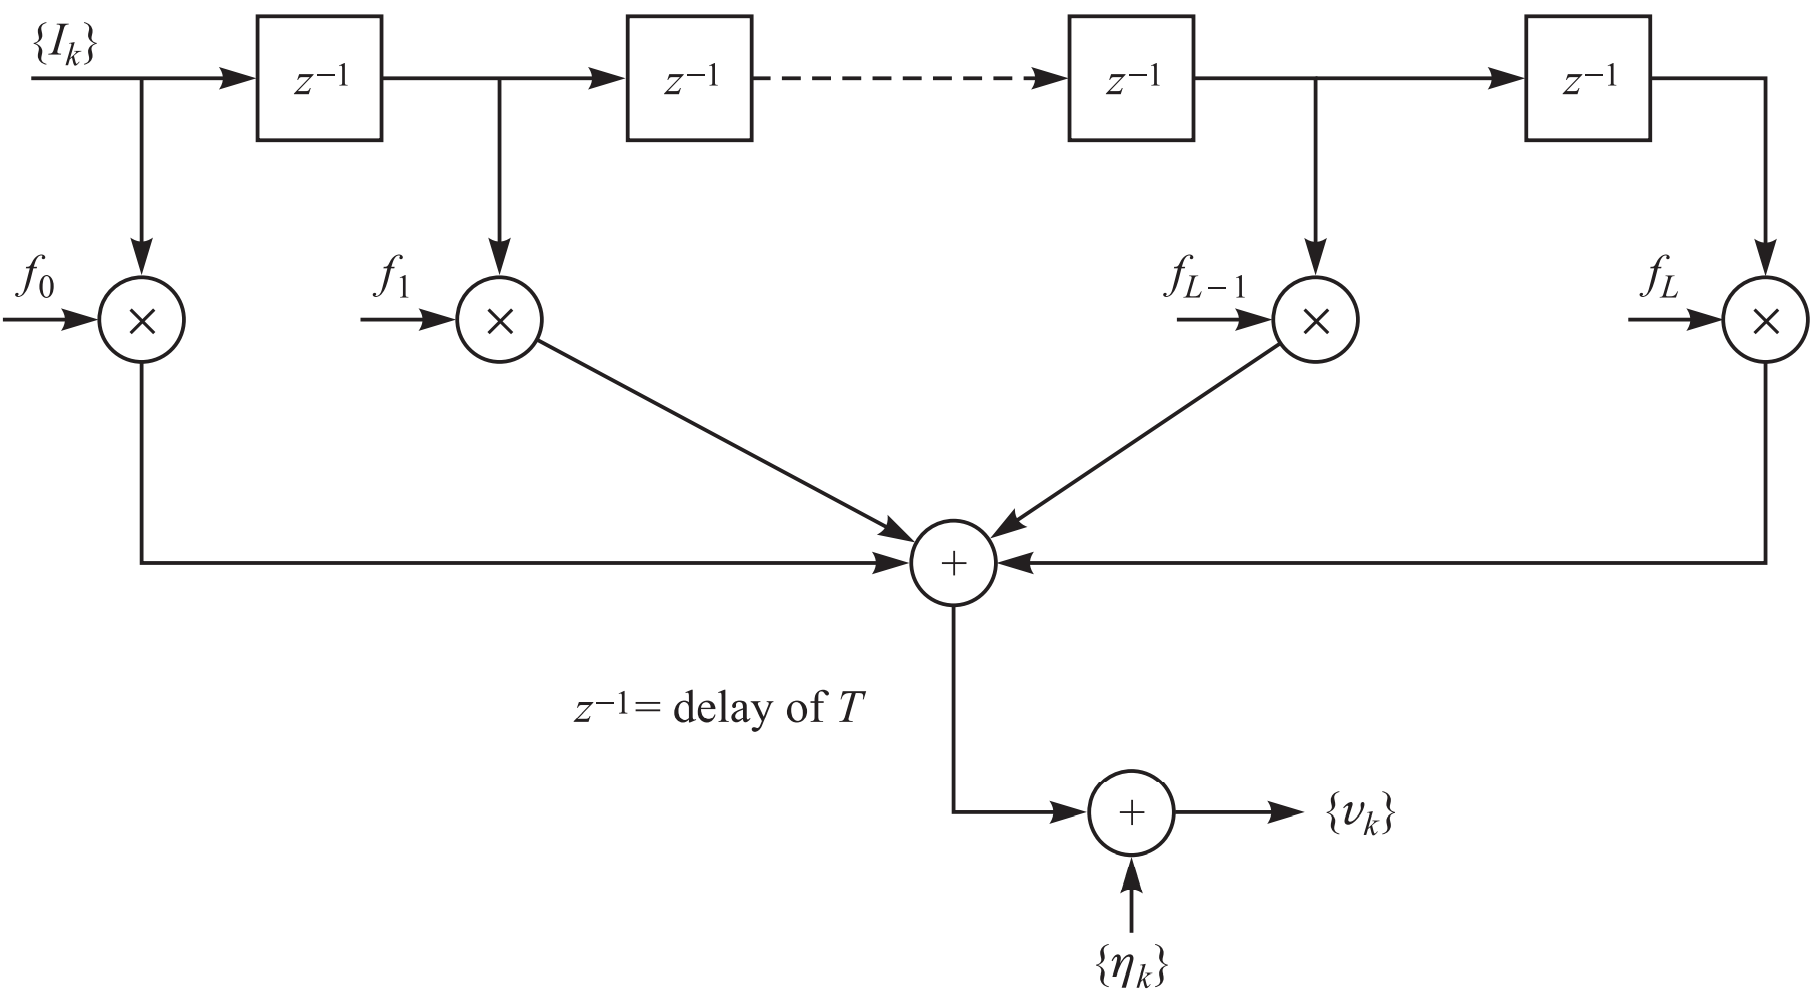
\includegraphics[scale=0.3]{Practice3-8-1.png}
            %     \caption{Equivalent discrete-time model of intersymbol interference channel with AWGN}
            % \end{figure}
            \begin{flushright}
                $\blacksquare$
            \end{flushright}
    %%%%%%%%%%%%%%%%%%%%%%%%%%%%%%%%%%%%%%%%%%%%%%
    \end{enumerate}
    \rule{\textwidth}{0.4pt}
\end{document}


